% Created 2021-12-19 Sun 17:22
\documentclass[9pt, b5paper]{article}
\usepackage[UTF8]{ctex}
\usepackage{xltxtra}
\usepackage{bera}
\usepackage[T1]{fontenc}
\usepackage[scaled]{beraserif}
\usepackage[scaled]{berasans}
\usepackage[scaled]{beramono}
\usepackage{graphicx}
\usepackage{xcolor}
\usepackage{multirow}
\usepackage{multicol}
\usepackage{float}
\usepackage{textcomp}
\usepackage{geometry}
\geometry{left=1.2cm,right=1.2cm,top=1.5cm,bottom=1.2cm}
\usepackage{algorithm}
\usepackage{algorithmic}
\usepackage{latexsym}
\usepackage{natbib}
\usepackage{minted}
\newminted{common-lisp}{fontsize=ootnotesize}
\usepackage[xetex,colorlinks=true,CJKbookmarks=true,linkcolor=blue,urlcolor=blue,menucolor=blue]{hyperref}
\author{deepwaterooo}
\date{\today}
\title{安卓中的线程、异步任务、Service与IntentService}
\hypersetup{
  pdfkeywords={},
  pdfsubject={},
  pdfcreator={Emacs 27.1 (Org mode 8.2.7c)}}
\begin{document}

\maketitle
\tableofcontents


\section{Java 创建线程的三种方式总结}
\label{sec-1}
\begin{itemize}
\item \url{https://blog.csdn.net/u011578734/article/details/110523825}
\end{itemize}
\subsection{继承 Thread 类}
\label{sec-1-1}
\begin{minted}[frame=lines,fontsize=\scriptsize,linenos=false]{java}
class MyThread extends Thread {
    @Override
        public void run() {
        super.run();
    }
}
private void testThread(){
    Thread thread = new MyThread();
    thread.start();
}
\end{minted}
\begin{itemize}
\item 缺点: Java 的单继承限制,想通过 Thread 实现多线程,就只能继承 Thread 类,不可继承其他类。
\end{itemize}
\subsection{实现 Runnable 接口}
\label{sec-1-2}
\begin{itemize}
\item 如果自己的类已经继承了其他类,这时就只能通过实现 Runnable 接口来实现多线程了。
\item 不过,继承 Runnable 接口后,想要启动线程,需要把该类的对象作为参数,传递给 Thread 的构造函数,并使用 Thread 类的实例方法 start 来启动。
\end{itemize}
\begin{minted}[frame=lines,fontsize=\scriptsize,linenos=false]{java}
public class TestThread extends A implements Runnable {
    public void run() {
        // todo
    }
}
// 启动线程
TestThread testThread = new TestThread();
Thread thread = new Thread(testThread);
thread.start();
\end{minted}
\begin{itemize}
\item Thread 内部的 run 方法我们可以看到它的实现原理:
\end{itemize}
\begin{minted}[frame=lines,fontsize=\scriptsize,linenos=false]{java}
private Runnable target;
public void run() {
    if (target != null) {
        target.run();
    }
}
\end{minted}
\begin{itemize}
\item target 是我们传递进来的 Runnable 对象,当线程执行时,线程的 run 方法会直接调用 Runnable 对象的 run 方法。
\end{itemize}
\subsection{实现 Callable 接口}
\label{sec-1-3}
\begin{itemize}
\item 如果想要执行的线程有返回,怎么处理呢?这时应该使用 Callable 接口了,与 Runnable 相比,Callable 可以有返回值,返回值通过 FutureTask 进行封装。
\end{itemize}
\begin{minted}[frame=lines,fontsize=\scriptsize,linenos=false]{java}
public class MyCallable implements Callable<Integer> {
    public Integer call() {
        return 111;
    }
}
public static void main(String[] args) throws ExecutionException, InterruptedException {
    MyCallable mc = new MyCallable();
    FutureTask<Integer> ft = new FutureTask<>(mc);
    Thread thread = new Thread(ft);
    thread.start();
    System.out.println(ft.get());
}
\end{minted}
\subsection{比较}
\label{sec-1-4}
\begin{itemize}
\item 这几种线程创建方式中,实现接口会更好一些,因为:
\begin{itemize}
\item Java 不支持多重继承,因此继承了 Thread 类就无法继承其它类,但是可以实现多个接口。
\item 类可能只要求可执行就行,继承整个 Thread 类开销过大。
\item 另外,如果需要有返回值时,使用 Callable 接口是适合的。
\end{itemize}
\end{itemize}


\section{Handler的使用}
\label{sec-2}
\begin{itemize}
\item Android中,不允许应用程序在子线程中更新UI,UI的处理必须在UI线程中进行,这样Android定制了一套完善的线程间通信机制——Handler通信机制。Handler作为Android线程通信方式,高频率的出现在我们的日常开发工作中,我们常用的场景包括:使用异步线程进行网络通信、后台任务处理等,Handler则负责异步线程与UI线程(主线程)之间的交互。
\item Android为了确保UI操作的线程安全,规定所有的UI操作都必须在主线程(UI线程)中执行,决定了UI线程中不能进行耗时任务,在开发过程中,需要将网络,IO等耗时任务放在工作线程中执行,工作线程中执行完成后需要在UI线程中进行刷新,因此就有了Handler进程内线程通信机制,当然Handler并不是只能用在UI线程与工作线程间的切换,Android中任何线程间通信都可以使用Handler机制。
\end{itemize}
\subsection{UI线程中使用Handler}
\label{sec-2-1}
\begin{itemize}
\item UI线程中使用Handler非常简单,因为框架已经帮我们初始化好了Looper,只需要创建一个Handler对象即可,之后便可以直接使用这个Handler实例向UI线程发消息(子线程--->UI线程)
\end{itemize}
\begin{minted}[frame=lines,fontsize=\scriptsize,linenos=false]{java}
    private Handler handler = new Handler(){
        @Override
        public void handleMessage(@NonNull Message msg) {
            super.handleMessage(msg);
            //处理消息
        }
    };
    @Override
    protected void onCreate(@Nullable Bundle savedInstanceState) {
        super.onCreate(savedInstanceState);
        setContentView(R.layout.activity_six);
    }
\end{minted}
\begin{itemize}
\item 这种方式会导致 \uline{内存泄露} 。
\item Handler 内存泄漏的两个原因: 
\begin{itemize}
\item Java 中非静态内部类和匿名内部类会持有外部类的引用
\end{itemize}
\end{itemize}
\begin{minted}[frame=lines,fontsize=\scriptsize,linenos=false]{java}
// 这是一个外部类 Handler 不会持有外部类引用
// 显然 handleMessage 没地方写了
Handler handler = new Handler();

// 重写 handleMessage 后将得到一个内部类 Handler,以内 handleMessage 是在外部类中实现的
// 它持有外部类引用,可能会引起内存泄漏
Handler handler = new Handler() { // 这是重写了handleMessage后的内部类Handler
  @Override public void handleMessage(Message msg) {
        super.handleMessage(msg);
        switch (msg.what) {
            case 0:
              MLog.i(msg.obj);
              break;
            case 1:
              break;
            default:

        }
    }
};

// 这里 Handler 是一个匿名类,但不是内部类
// Runnable 是一个匿名内部类,持有外部类引用,可能会引起内存泄漏
new Handler().post(new Runnable() {
    @Override public void run() {
      // ...
    }
});
\end{minted}
\begin{itemize}
\item Handler 的生命周期比外部类长
\item 我们通过Handler发送消息,在Message对象中会持有当前Handler对象的引用,在Java中非静态成员类、内部类、匿名类会持有外部对象的引用(这里在源码中有提到),而Looper是线程局部变量,其生命周期与UI线程相同,Looper持有MessageQueue的引用,MessageQueue持有Message的引用,当通过Handler发送一个延时消息未处理之前用户已经离开当前Activity,会导致Activity不能及时释放而内存泄漏。
\item 分析
\begin{itemize}
\item 非静态的内部 Handler 子类、匿名 Handler 子类会持有外部类的引用(Activity),而 Handler 可能会因为要等待处理耗时操作导致存活时间超过 Activity,或者消息队列中存在未被 Looper 处理的 Message ,而 Message 会持有 Handler 的引用。于是,在 Activity 退出时,其引用还是被 Handler 持有,导致 Activity 无法被及时回收,造成内存泄露。
\item 非静态的内部 Runnable 子类、匿名 Runnable 子类 post 到任意 Handler 上时,Runnable 其实是 Massage中的 Callback,持有 Message 引用,如果这个 Massage 在消息队列还没有被处理,那么就会造成 Runnable 一直持有外部类的引用而造成内存泄露。
\end{itemize}
\end{itemize}
\subsubsection{解决思路}
\label{sec-2-1-1}
\begin{itemize}
\item 通过静态内部类或者外部类来声明 Handler 和 Runnable,然后使用弱引用来拿到外部类的变量。
\item 在 Activity/Fragment 销毁的时候请空 MessageQueue 中的消息。
\end{itemize}
\begin{enumerate}
\item 官方推荐的一种
\label{sec-2-1-1-1}
\begin{minted}[frame=lines,fontsize=\scriptsize,linenos=false]{java}
private Handler handler = new Handler(new Handler.Callback() {
        @Override
        public boolean handleMessage(@NonNull Message msg) {
            switch (msg.what){
            case 1:
            //处理子线程发过来的消息
            Toast.makeText(SixActivity.this,(String)msg.obj,Toast.LENGTH_LONG).show();
            Log.d("aa",(String) msg.obj);
            break;

            }
            return false;
        }
    });
\end{minted}
\item 静态内部类
\label{sec-2-1-1-2}
\begin{itemize}
\item 下面的例子实现了子线程(执行run()耗时函数的线程)向主线程发送消息
\begin{minted}[frame=lines,fontsize=\scriptsize,linenos=false]{java}
public static final int LOAD_COM = 1; // 加载任务的id标志

private Handler mHandler = new MyHandler(MainActivity.this); // 在MainActivity中,创建了一个Handler对象。

private static class MyHandler extends Handler { // MainActivity中的静态static内部类
    private final WeakReference<MainActivity> mActivity; // 持有当前MainActivity的WeakReference
    private MyHandler(MainActivity activity) {
        this.mActivity = new WeakReference(activity);
    }
    @Override public void handleMessage(@NonNull Message msg) { // ui线程中,负责消息返回的处理逻辑
        super.handleMessage(msg);      // UI线程中,Handler对象的handleMessage方法负责处理消息的返回
        switch (msg.what){
        case LOAD_COM:
            Log.d("TestHandler", msg.obj.toString());
            MainActivity mainActivity = mActivity.get();
            if (mainActivity != null){
                mainActivity.mTextView.setText(msg.obj.toString());
            }
            break;
        }
    }
};
@Override public void onClick(View v) {
    switch (v.getId()) {
    case R.id.start_load: // 当按钮start_load点击时,启动一个后台线程,模拟一个后台加载过程(线程休眠1秒)
        new Thread() {
            @Override
            public void run() { // 后台线程中执行的逻辑:这里代码写定义在主线程MainActivity中,但实际run()函数的真正执行是执行在子线程中
                try {
                    Thread.sleep(1000);
                } catch (InterruptedException e) {
                    e.printStackTrace();
                }
// 子线程发送消息
                // Message message = new Message();//可以使用new Message来创建消息,但是一般不这样使用?
                Message message = Message.obtain(); // 后台任务完成后,使用Handler对象的sendMessage方法发送消息(一个Messaage对象)给UI线程
                message.what = LOAD_COM;
                message.obj = "我是子线程消息";
                mHandler.sendMessage(message); // 从后台线程中,发送消息给UI线程
            }
        }.start();
        break;
    }
}
\end{minted}
\item 主线程给子线程发送消息(UI线程--->子线程)
\begin{minted}[frame=lines,fontsize=\scriptsize,linenos=false]{java}
public class SixActivity extends AppCompatActivity {
    private Handler handler;
    private Button btn;
    @Override
        protected void onCreate(@Nullable Bundle savedInstanceState) {
        super.onCreate(savedInstanceState);
        setContentView(R.layout.activity_six);
        new MyOneThread().start();     // 子线程创建方式
        btn= findViewById(R.id.dian);
        btn.setOnClickListener(new View.OnClickListener() {
                @Override
                    public void onClick(View v) {
                    Message message=Message.obtain();
                    message.what=1;
                    message.obj = "我是主线程的消息发送给子线程";
                    handler.sendMessage(message); // 封装完数据发送给子线程
                }
            });
    }
    class MyOneThread extends Thread {
        @Override public void run() {
            // 在子线程中处理消息,子线程中处理消息,没有默认的Loop
            // 由于只有主线程成才默认的Looper.prepare(), Looper.loop();
            Looper.prepare(); // 创建Looper: 如果不添加会报错
            handler = new Handler() { // 在子线程中创建消息Handler
                @Override
                public void handleMessage(@NonNull Message msg) {
                    switch (msg.what){
                    case 1:
                    Log.d("aa",(String) msg.obj);
                    break;
                    }
                }
            };
            // 循环读取messageQueue
            Looper.loop(); // 如果不添加读取不到消息
        }
    }
}
\end{minted}
\item 子线程中,也可以使用这个方式来获取Looper
\end{itemize}
\begin{minted}[frame=lines,fontsize=\scriptsize,linenos=false]{java}
handler = new Handler(Looper.getMainLooper()) {
    @Override
    public void handleMessage(@NonNull Message msg) {
        switch (msg.what) {
        case 1:
        Log.d("aa",(String) msg.obj);
        break;
        }
    }
};
\end{minted}
\begin{itemize}
\item 子线程发送消息到子线程(子线程----->子线程)
\end{itemize}
\begin{minted}[frame=lines,fontsize=\scriptsize,linenos=false]{java}
btn.setOnClickListener(new View.OnClickListener() {
        @Override public void onClick(View v) {
            new Thread(new Runnable() {
                    @Override
                    public void run() {
                        Message message = Message.obtain();
                        message.obj = "我是子线程发送到子线消息";
                        message.what = 1;
                        handler.sendMessage(message); // 发送消息的子线程也是有handler的
                    }
                }).start();
        }
    });
class MyOneThread extends Thread {
    @Override public void run() {
        //在子线程中处理消息,子线程中处理消息,没有默认的Loop
        //由于只有主线程成才默认的Looper.prepare(), Looper.loop();
        // Looper.prepare(); // 创建Looper: 效果一样,换下面的方式
        handler = new Handler(Looper.getMainLooper()){
            @Override
            public void handleMessage(@NonNull Message msg) {
                switch (msg.what){
                case 1:
                Log.d("aa",(String) msg.obj);
                break;
                }
            }
        };
        // Looper.loop(); // 循环读取messageQueue
    }
}
\end{minted}
\begin{itemize}
\item 使用Handler.post()直接更新ui
\end{itemize}
\begin{minted}[frame=lines,fontsize=\scriptsize,linenos=false]{java}
private Handler handler=new Handler();
@Override
protected void onCreate(@Nullable Bundle savedInstanceState) {
    super.onCreate(savedInstanceState);
    setContentView(R.layout.activity_six);
    btn = findViewById(R.id.dian);
    new Thread(new Runnable() {
            @Override
            public void run() {
                // Message message=Message.obtain();
                // message.obj="我是子线程静态消息";
                // message.what=1;
                // handler.sendMessage(message);
                handler.post(new Runnable() {
                        @Override
                        public void run() {
                            Log.d("aa","直接更新Ui");
                            btn.setText("我是更新的消息");
                        }
                    });
            }
        }).start();
}
\end{minted}
\begin{itemize}
\item post和sendMessage本质上是没有区别的,只是实际用法中有一点差别
\item post也没有独特的作用,post本质上还是用sendMessage实现的,post只是一中更方便的用法而已
\end{itemize}

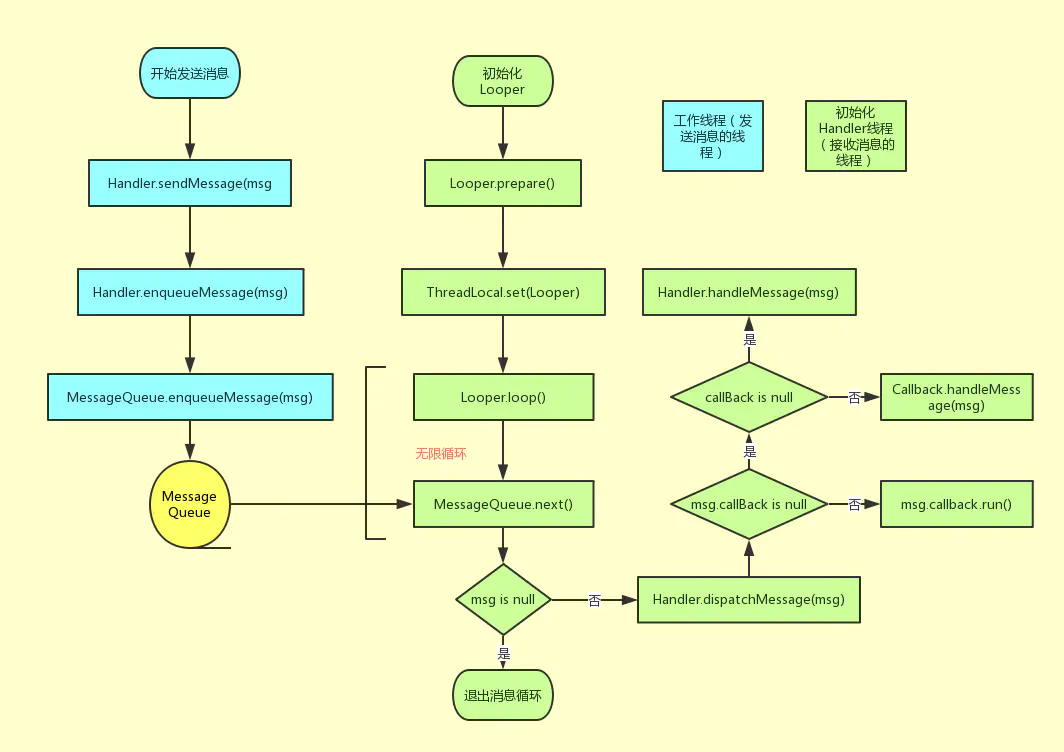
\includegraphics[width=.9\linewidth]{./pic/handler.png}
\end{enumerate}

\subsection{关于安卓handler的面试小问题}
\label{sec-2-2}
\subsubsection{Looper和Handler一定要处于一个线程吗?子线程中可以用MainLooper去创建Handler吗?}
\label{sec-2-2-1}
\begin{itemize}
\item (1)子线程中
\end{itemize}
\begin{minted}[frame=lines,fontsize=\scriptsize,linenos=false]{java}
Handler handler = new Handler(Looper.getMainLooper()); // 此时,子线程的handler与Looper.getMainLooper()主线程Looper, 两者就不在一个线程中
\end{minted}
\begin{itemize}
\item 此时两者就不在一个线程中
\item (2)子线程中可以用MainLooper去创建Handler.
\end{itemize}
\subsubsection{Handler的post方法发送的是同步消息吗?可以发送异步消息吗?}
\label{sec-2-2-2}
\begin{itemize}
\item 用户层面发送的都是同步消息
\item 不能发送异步消息
\item 异步消息只能由系统发送。
\end{itemize}
\subsubsection{Handler.post的逻辑在哪个线程执行的,是由Looper所在线程还是Handler所在线程决定的?}
\label{sec-2-2-3}
\begin{itemize}
\item 由Looper所在线程决定的
\item 最终逻辑是在Looper.loop()方法中,从MsgQueue中拿出msg,并且执行其逻辑,这是在Looper中执行的,因此是由Looper所在的线程决定的。
\end{itemize}
\subsubsection{Handler构造方法中通过Looper.myLooper();是如何获取到当前线程的Looper的?}
\label{sec-2-2-4}
\begin{itemize}
\item myLooper()内部使用ThreadLocal实现,因此能够获取各个线程自己的Looper
\end{itemize}
\subsubsection{MessageQueue(消息队列)}
\label{sec-2-2-5}
\begin{itemize}
\item 消息队列被封装到Looper里面了,我们一般不会直接与MessageQueue打交道。我们只需要记住它是用来存放消息的单链表结构。队列的顺序由Message的next属性来维护。MessageQueue是整个Handler机制的核心,里面涉及很多特性我们这里都不展开讲述(比如消息屏障机制)。
\end{itemize}

\subsection{handler工作原理总结: Handler的工作原理}
\label{sec-2-3}
\begin{itemize}
\item Handler机制整体流程;
\begin{itemize}
\item IdHandler(闲时机制);
\item postDelay()的具体实现;
\item post()与sendMessage()区别;
\item 使用Handler需要注意什么问题,怎么解决的?
\end{itemize}
\item 问题很细,能准备多详细就准备多详细。人家自己封装了一套 Handler 来避免内存泄漏问题
\item Handler的消息传递机制涉及到四个部分:
\begin{itemize}
\item 1. Message:线程间传递的对象。
\item 2. MessageQueue: 消息队列,用来存放Handler发布的Message.
\item 3. Handler:负责将Message插入到MessageQueue中以及对MessageQueue中的Message进行处理。
\item 4. Looper:负责从MessageQueue中取出Message,并交给Handler.
\end{itemize}
\item 其中:
\begin{itemize}
\item Looper存储在ThreadLocal中,Looper在创建时会同时创建MessageQueue,作为其成员对象.因此Looper和MessageQueue是属于创建者线程的,各线程之间的Looper和MessageQueue相互独立。
\item Handler在创建时会从当前线程的ThreadLocal中取得Looper.
\item 发送消息时,在发送线程中调用接收线程中的Handler的sendMessage方法,过程中,Handler会将自身赋予到Message的target中,并将Message插入到Handler对应的MessageQueue中。
\item 而接收线程中的Looper在循环过程中会取出这个Message,通过Message.target取出接收线程中的Handler,并将消息交Handler对象处理。由此实现了跨线程通信。
\item 要注意的是:线程与Looper和MessageQueue是一对一的关系,即一个线程只维护一个Looper和一个MessageQueue;而线程与Handler的关系是一对多,即一个线程可以有很多Handler,一个Handler只对应一个线程,这也是为什么Handler在发送消息时,为什么要将自身赋给Message.target的原因。
\end{itemize}
\item Handler内存泄露的解决方法
\begin{itemize}
\item 方法1:通过程序逻辑进行保护。
\begin{itemize}
\item 关闭Activity的时候停掉后台线程,这样就相当于切断了Handler和外部连接的线,Activity自然会在合适的时候被回收。
\item 如果你的Handler是被delay的Message持有了引用,那么在Activity销毁前使用相应的Handler的removeCallbacksAndMessages()方法,把消息对象从消息队列移除就行了。
\end{itemize}
\item 方法2:将Handler声明为静态类
\begin{itemize}
\item 静态类不持有外部类的对象,这样即使Handler在运行,Activity也可以被回收。
\item 由于静态类的Handler不再持有外部类对象,如果要操作Activity需要增加一个Activity的弱引用。
\end{itemize}
\end{itemize}
\item 优点:
\begin{itemize}
\item 操作简单,无学习成本。
\end{itemize}
\item 缺点:
\begin{itemize}
\item 代码规范性较差,不易维护。
\item 每次操作都会开启一个匿名线程,系统开销较大。
\end{itemize}
\end{itemize}
\subsubsection{Looper.loop()为什么不会阻塞主线程?}
\label{sec-2-3-1}
\begin{itemize}
\item \url{https://segmentfault.com/a/1190000037449196} 这部分格式再整理一下
\end{itemize}
主线程Looper从消息队列读取消息,当读完所有消息时,主线程阻塞。子线程往消息队列发送消息,并且往管道文件写数据,主线程即被唤醒,从管道文件读取数据,主线程被唤醒只是为了读取消息,当消息读取完毕,再次睡眠。因此loop的循环并不会对CPU性能有过多的消耗。

主线程中如果没有looper进行循环,那么主线程一运行完毕就会退出。那么我们还能运行APP吗,显然,这是不可能的,Looper主要就是做消息循环,然后由Handler进行消息分发处理,一旦退出消息循环,那么你的应用也就退出了。

总结:Looper的无限循环必不可少。

补充说明:

我看有一部分人理解”Looper.loop()的阻塞“和”UI线程上执行耗时操作卡死“的区别时还一脸懵逼的状况,简单回答一波:

首先这两之间一点联系都没有,完全两码事。
Looper上的阻塞,前提是没有输入事件,MsgQ为空,Looper空闲状态,线程进入阻塞,释放CPU执行权,等待唤醒。
UI耗时导致卡死,前提是要有输入事件,MsgQ不为空,Looper正常轮询,线程并没有阻塞,但是该事件执行时间过长(5秒?),而且与此期间其他的事件(按键按下,屏幕点击..)都没办法处理(卡死),然后就ANR异常了。
\subsubsection{Android -- Looper.prepare()和Looper.loop() —深入版}
\label{sec-2-3-2}
Android中的Looper类,是用来封装消息循环和消息队列的一个类,用于在android线程中进行消息处理。handler其实可以看做是一个工具类,用来向消息队列中插入消息的。

​ (1) Looper类用来为一个线程开启一个消息循环。 默认情况下android中新诞生的线程是没有开启消息循环的。(主线程除外,主线程系统会自动为其创建Looper对象,开启消息循环。) Looper对象通过MessageQueue来存放消息和事件。一个线程只能有一个Looper,对应一个MessageQueue。

(2) 通常是通过Handler对象来与Looper进行交互的。Handler可看做是Looper的一个接口,用来向指定的Looper发送消息及定义处理方法。 默认情况下Handler会与其被定义时所在线程的Looper绑定,比如,Handler在主线程中定义,那么它是与主线程的Looper绑定。 mainHandler = new Handler() 等价于new Handler(Looper.myLooper()). Looper.myLooper():获取当前进程的looper对象,类似的 Looper.getMainLooper() 用于获取主线程的Looper对象。

(3) 在非主线程中直接new Handler() 会报如下的错误:

E/AndroidRuntime( 6173): Uncaught handler: thread Thread-8 exiting due to uncaught exception E/AndroidRuntime( 6173): java.lang.RuntimeException: Can't create handler inside thread that has not called Looper.prepare()

原因是非主线程中默认没有创建Looper对象,需要先调用Looper.prepare()启用Looper。

(4) Looper.loop();

让Looper开始工作,从消息队列里取消息,处理消息。

注意:写在Looper.loop()之后的代码不会被执行,这个函数内部应该是一个循环,当调用mHandler.getLooper().quit()后,loop才会中止,其后的代码才能得以运行。
(5) 基于以上知识,可实现主线程给子线程(非主线程)发送消息。

\subsubsection{线程的切换又是怎么回事?}
\label{sec-2-3-3}
那么线程的切换又是怎么回事呢?
很多人搞不懂这个原理,但是其实非常简单,我们将所涉及的方法调用栈画出来,如下:

Thread.foo()\{
    Looper.loop()
     -> MessageQueue.next()
      -> Message.target.dispatchMessage()
       -> Handler.handleMessage()
\}
显而易见,Handler.handleMessage() 所在的线程最终由调用 Looper.loop() 的线程所决定。

平时我们用的时候从异步线程发送消息到 Handler,这个 Handler 的 handleMessage() 方法是在主线程调用的,所以消息就从异步线程切换到了主线程。
\subsubsection{Handler是如何实现线程之间的切换的}
\label{sec-2-3-4}
Handler是如何实现线程之间的切换的呢?例如现在有A、B两个线程,在A线程中有创建了handler,然后在B线程中调用handler发送一个message。

通过上面的分析我们可以知道,当在A线程中创建handler的时候,同时创建了MessageQueue与Looper,Looper在A线程中调用loop进入一个无限的for循环从MessageQueue中取消息,当B线程调用handler发送一个message的时候,会通过msg.target.dispatchMessage(msg);将message插入到handler对应的MessageQueue中,Looper发现有message插入到MessageQueue中,便取出message执行相应的逻辑,因为Looper.loop()是在A线程中启动的,所以则回到了A线程,达到了从B线程切换到A线程的目的。

image

小结:

1.Handler初始化之前,Looper必须初始化完成。UI线程之所以不用初始化,因为在ActivityThread已经初始化,其他子线程初始化Handler时,必须先调用Looper.prepare()。

2.通过Handler发送消息时,消息会回到Handler初始化的线程,而不一定是主线程。

3.使用ThreadLocal时,需要注意内存泄漏的问题。

通俗点的说法Handler机制其实就是借助共享变量来进行线程切换的.

Handler是如何实现线程之间的切换的

妙用 Looper 机制

我们可以利用 Looper 的机制来帮助我们做一些事情:

将 Runnable post 到主线程执行;
利用 Looper 判断当前线程是否是主线程。
完整示例代码如下:

public final class MainThread \{

private MainThread() \{
\}

private static final Handler HANDLER = new Handler(Looper.getMainLooper());

public static void run(@NonNull Runnable runnable) \{
    if (isMainThread()) \{
        runnable.run();
    \}else\{
        HANDLER.post(runnable);
    \}
\}

public static boolean isMainThread() \{
    return Looper.myLooper() == Looper.getMainLooper();
\}

\}
能够省去不少样板代码。
先明确我们的问题:

Handler 是如何与线程关联的?
Handler 发出去的消息是谁管理的?
消息又是怎么回到 handleMessage() 方法的?
线程的切换是怎么回事?
回答:Handler 发送的消息由 MessageQueue 存储管理,并由 Loopler 负责回调消息到 handleMessage()。

线程的转换由 Looper 完成,handleMessage() 所在线程由 Looper.loop() 调用者所在线程决定。
\subsubsection{为什么在子线程中创建 Handler 会抛异常}
\label{sec-2-3-5}
\begin{itemize}
\item Handler 的工作是依赖于 Looper 的,而 Looper(与消息队列)又是属于某一 个线程(ThreadLocal 是线程内部的数据存储类,通过它可以在指定线程中存储 数据,其他线程则无法获取到),其他线程不能访问。因此 Handler 就是间接 跟线程是绑定在一起了。因此要使用 Handler 必须要保证 Handler 所创建的线 程中有 Looper 对象并且启动循环。因为子线程中默认是没有 Looper 的,所以 会报错。 正确的使用方法是:
\end{itemize}
\begin{minted}[frame=lines,fontsize=\scriptsize,linenos=false]{java}
public class WorkThread extends Thread {
    private Handler mHander;
    public Handler getHander() {
        return mHander;
    }
    public void quit() { // 这里是资源释放吗?
        mHander.getLooper().quit();
    }
    @Override
        public void run() {
        super.run();

        // 创建该线程对应的 Looper,
        // 内部实现
        //   1。new Looper()
        //   2。将 1 步中的 lopper 放在 ThreadLocal 里,ThreadLocal 是保存数据的, 主要应用场景是:线程间数据互不影响的情况
        //   3。在 1 步中的 Looper 的构造函数中 new MessageQueue();
        // 对消息机制不懂得同学可以查阅资料,网上很多也讲的很不错。
        Looper.myLooper(); // 一般是call Looper.prepare();吧,再查一下

        mHander = new Handler(){
            @SuppressLint("HandlerLeak")
            @Override
            public void handleMessage(Message msg) {
                super.handleMessage(msg);
                Log.d("WorkThread", (Looper.getMainLooper() == Looper.myLooper()) + "," + msg.what);
            }
        };
        
        // 注意这 3 个的顺序不能颠倒
        Looper.loop();
    }
}
\end{minted}
\subsubsection{Handler发送延时消息}
\label{sec-2-3-6}
\begin{itemize}
\item handler发送延时消息是通过postDelayed()方法将Runnanle对象封装成Message,然后调用sendMessageAtTime(),设置的时间是当时的时间+延时的时间。
\item 发送延时消息实际上是往messageQueue中加入一条Message。
\item Message在MessageQueue中实际是以单链表来存储的,且是按照时间顺序来插入的。时间顺序是以Message中的when属性来排序的。
\item 重点:
\begin{itemize}
\item postDelay并不是等待delayMillis延时时常后再加入消息队列,而是加入消息队列后阻塞(消息队列会按照阻塞时间排序)等待delayMillis后唤醒消息队列再执行。
\item sleep会阻塞线程
\item postDelayed不会阻塞线程
\end{itemize}
\end{itemize}
\subsubsection{Handler线程间通信}
\label{sec-2-3-7}
\begin{itemize}
\item 作用:线程之间的消息通信
\item 流程:主线程默认实现了Looper (调用loop.prepare方法 向sThreadLocal中set一个新的looper对象, looper构造方法中又创建了MsgQueue) 手动创建Handler ,调用 sendMessage 或者 post (runable) 发送Message 到 msgQueue ,如果没有Msg 这添加到表头,有数据则判断when时间 循环next 放到合适的 msg的next 后。Looper.loop不断轮训Msg,将msg取出 并分发到Handler 或者 post提交的 Runable 中处理,并重置Msg 状态位。回到主线程中 重写 Handler 的 handlerMessage 回调的msg 进行主线程绘制逻辑。
\item 问题:
\begin{itemize}
\item Handler 同步屏障机制:通过发送异步消息,在msg.next 中会优先处理异步消息,达到优先级的作用
\item Looper.loop 为什么不会卡死:为了app不挂掉,就要保证主线程一直运行存在,使用死循环代码阻塞在msgQueue.next()中的nativePollOnce()方法里 ,主线程就会挂起休眠释放cpu,线程就不会退出。Looper死循环之前,在ActivityThread.main()中就会创建一个 Binder 线程(ApplicationThread),接收系统服务AMS发送来的事件。当系统有消息产生(其实系统每 16ms 会发送一个刷新 UI 消息唤醒)会通过epoll机制 向pipe管道写端写入数据 就会发送消息给 looper 接收到消息后处理事件,保证主线程的一直存活。只有在主线程中处理超时才会让app崩溃 也就是ANR。
\item Messaage复用: 将使用完的Message清除附带的数据后, 添加到复用池中 ,当我们需要使用它时,直接在复用池中取出对象使用,而不需要重新new创建对象。复用池本质还是Message 为node 的单链表结构。所以推荐使用Message.obation获取 对象。
\end{itemize}
\end{itemize}

\section{AsyncTask}
\label{sec-3}
\begin{itemize}
\item 较为轻量级的异步类,封装了 FutureTask 的线程池、ArrayDeque 和 Handler 进行调度。AsyncTask 主要用于 \uline{后台与界面持续交互}
\item 我们来看看 AsyncTask 这个抽象类的定义,当我们定义一个类来继承 AsyncTask 这个类的时候,我们需要为其指定3个泛型参数:
\end{itemize}
\begin{minted}[frame=lines,fontsize=\scriptsize,linenos=false]{java}
AsyncTask <Params, Progress, Result>
\end{minted}
\begin{itemize}
\item Params: 这个泛型指定的是我们传递给异步任务执行时的参数的类型。
\item Progress: 这个泛型指定的是我们的异步任务在执行的时候将执行的进度返回给UI线程的参数的类型。
\item Result: 这个泛型指定的异步任务执行完后返回给UI线程的结果的类型。
\item 我们在定义一个类继承 AsyncTask 类的时候,必须要指定好这三个泛型的类型,如果都不指定的话,则都将其写成 void。
\item 我们来看一个官方给的例子:
\end{itemize}
\begin{minted}[frame=lines,fontsize=\scriptsize,linenos=false]{java}
private class DownloadFilesTask extends AsyncTask<URL, Integer, Long> {
     protected Long doInBackground(URL... urls) {
         int count = urls.length;
         long totalSize = 0;
         for (int i = 0; i < count; i++) {
             totalSize += Downloader.downloadFile(urls[i]);
             publishProgress((int) ((i / (float) count) * 100));
             // Escape early if cancel() is called
             if (isCancelled()) break;
         }
         return totalSize;
     }
     protected void onProgressUpdate(Integer... progress) {
         setProgressPercent(progress[0]);
     }
     protected void onPostExecute(Long result) {
         showDialog("Downloaded " + result + " bytes");
     }
}
\end{minted}
\begin{itemize}
\item 使用时只需要集成 AsyncTask,创建对象并调用 execute 执行即可:
\end{itemize}
\begin{minted}[frame=lines,fontsize=\scriptsize,linenos=false]{java}
new DownloadFilesTask().execute(url1, url2, url3);
\end{minted}
\begin{itemize}
\item doInBackground(Params…) 方法里执行耗时逻辑,然后在 onPostExecute(Result) 中将结果更新回UI组件
\item AsyncTask 的几个主要方法中,doInBackground 方法运行在子线程,execute、onPreExecute、onProgressUpdate、onPostExecute 这几个方法都是在 UI 线程运行的。
\end{itemize}
\subsection{使用 AsyncTask 的注意事项}
\label{sec-3-1}
\begin{itemize}
\item AsyncTask 的实例必须在 UI Thread 中创建。
\item 只能在 UI 线程中调用 AsyncTask 的 execute 方法。
\item AsyncTask 被重写的四个方法是系统自动调用的,不应手动调用。
\item 每个AsyncTask 只能被执行一次,多次执行会引发异常。
\item AsyncTask 的四个方法,只有 doInBackground 方法是运行在其他线程中,其他三个方法都运行在 UI 线程中,也就说其他三个方法都可以进行 UI 的更新操作。
\item AsyncTask 默认是串行执行,如果需要并行执行,使用接口 executeOnExecutor 方法。
\end{itemize}
\subsection{优点:}
\label{sec-3-2}
\begin{itemize}
\item 结构清晰,使用简单,适合后台任务的交互。
\item 异步线程的优先级已经被默认设置成了:THREAD$_{\text{PRIORITY}}$$_{\text{BACKGROUND,不会与}}$ UI 线程抢占资源。
\end{itemize}
\subsection{缺点:}
\label{sec-3-3}
\begin{itemize}
\item 结构略复杂,代码较多。
\item 每个 AsyncTask 只能被执行一次,多次调用会发生异常。
\item AsyncTask 在整个 Android 系统中维护一个线程池,有可能被其他进程的任务抢占而降低效率。
\end{itemize}

\section{HandlerThread}
\label{sec-4}
\begin{itemize}
\item HandlerThread 是一个自带 Looper 消息循环的线程类。处理异步任务的方式和 Thread + Looper + Handler 方式相同。
\end{itemize}
\subsection{优点:}
\label{sec-4-1}
\begin{itemize}
\item 简单,内部实现了普通线程的 Looper 消息循环。
\item 可以串行执行多个任务。
\item 内部拥有自己的消息队列,不会阻塞 UI 线程。
\end{itemize}
\subsection{缺点:}
\label{sec-4-2}
\begin{itemize}
\item 没有结果返回接口,需要自行处理。
\item 消息过多时,容易造成阻塞。
\item 只有一个线程处理,效率较低。
\item 线程优先级默认优先级为 THREAD$_{\text{PRIORITY}}$$_{\text{DEFAULT,容易和}}$ UI 线程抢占资源。
\end{itemize}

\section{IntentService}
\label{sec-5}
\begin{itemize}
\item IntentService 继承自 Service 类,用于启动一个异步服务任务,它的内部是通过 HandlerThread 来实现异步处理任务的。
\item 我们来看下 IntentService 的主要方法:
\end{itemize}
\begin{minted}[frame=lines,fontsize=\scriptsize,linenos=false]{java}
// mServiceLooper;
// mServiceHandler;
@Override
public void onCreate() {
    // TODO: It would be nice to have an option to hold a partial wakelock during processing,
    // and to have a static startService(Context, Intent) method that would launch the service & hand off a wakelock.
    super.onCreate();
    HandlerThread thread = new HandlerThread("IntentService [" + mName + "]");
    thread.start();
    mServiceLooper = thread.getLooper();
    mServiceHandler = new ServiceHandler(mServiceLooper);
}
@Override
public void onStart(@Nullable Intent intent, int startId) {
    Message msg = mServiceHandler.obtainMessage();
    msg.arg1 = startId;
    msg.obj = intent;
    mServiceHandler.sendMessage(msg);
}
private final class ServiceHandler extends Handler {
    public ServiceHandler(Looper looper) {
        super(looper);
    }
    @Override
        public void handleMessage(Message msg) {
        onHandleIntent((Intent)msg.obj);
        stopSelf(msg.arg1);
    }
}
\end{minted}
\subsection{优点:}
\label{sec-5-1}
\begin{itemize}
\item 只需要继承 IntentService,就可以在 onHandlerIntent 方法中异步处理 Intent 类型任务了。
\item 任务结束后 IntentService 会自行停止,无需手动调用 stopService。
\item 可以执行处理多个 Intent 请求,顺序执行多任务。
\item IntentService 是继承自 Service,具有后台 Service 的优先级。
\end{itemize}
\subsection{缺点:}
\label{sec-5-2}
\begin{itemize}
\item 需要启动服务来执行异步任务,不适合简单任务处理。
\item 异步任务是由 HandlerThread 实现的,只能单线程、顺序处理任务。
\item 没有返回 UI 线程的接口。
\end{itemize}

\section{使用线程池来处理异步任务}
\label{sec-6}
\begin{itemize}
\item 利用 Executors 的静态方法 newCachedThreadPool()、newFixedThreadPool()、newSingleThreadExecutor() 及重载形式实例化 ExecutorService 接口即得到线程池对象。
\item 动态线程池 newCachedThreadPool():根据需求创建新线程的,需求多时,创建的就多,需求少时,JVM 自己会慢慢的释放掉多余的线程。
\item 固定数量的线程池 newFixedThreadPool():内部有个任务阻塞队列,假设线程池里有2个线程,提交了4个任务,那么后两个任务就放在任务阻塞队列了,即使前2个任务 sleep 或者堵塞了,也不会执行后两个任务,除非前2个任务有执行完的。
\item 单线程 newSingleThreadExecutor():单线程的线程池,这个线程池可以在线程死后(或发生异常时)重新启动一个线程来替代原来的线程继续执行下去。
\end{itemize}
\subsection{优点:}
\label{sec-6-1}
\begin{itemize}
\item 线程的创建和销毁由线程池来维护,实现了线程的复用,从而减少了线程创建和销毁的开销。
\item 适合执行大量异步任务,提高性能。
\item 灵活性高,可以自由控制线程数量。
\item 扩展性好,可以根据实际需要进行扩展。
\end{itemize}
\subsection{缺点:}
\label{sec-6-2}
\begin{itemize}
\item 代码略显复杂。
\item 线程池本身对系统资源有一定消耗。
\item 当线程数过多时,线程之间的切换成本会有很大开销,从而使性能严重下降。
\item 每个线程都会耗费至少 1040KB 内存,线程池的线程数量需要控制在一定范围内。
\item 线程的优先级具有继承性,如果在 UI 线程中创建线程池,线程的默认优先级会和 UI 线程相同,从而对 UI 线程使用资源进行抢占。
\end{itemize}
% Emacs 27.1 (Org mode 8.2.7c)
\end{document}